\section{Consuntivi di periodo}
Di seguito vengono indicate le spese sostenute per ogni ruolo, confrontate con quanto preventivato. Il bilancio potrà essere:
\begin{itemize}
\item \textbf{positivo}: se la spesa effettiva è minore di quanto preventivato;
\item \textbf{pari}: se la spesa effettiva è uguale a quanto preventivato;
\item \textbf{negativo}: se la spesa effettiva è maggiore di quanto preventivato.
\end{itemize}

\subsection{Fase di Analisi}
\subsubsubsection{Consuntivo}
Le ore di lavoro impiegate nella fase di analisi vengono considerate come ore di investimento; per questo motivo non verranno rendicontate.

\begin{table}[H]
\begin{center}
\rowcolors{2}{gray!25}{white}
\renewcommand{\arraystretch}{1.5}
\begin{tabular}{ m{0.16\textwidth}<{\centering}  m{0.12\textwidth}<{\centering} m{0.12\textwidth}<{\centering} m{0.14\textwidth}<{\centering} m{0.16\textwidth}<{\centering} m{0.14\textwidth}<{\centering}}	\rowcolor{darkblue}
	\textcolor{white}{\textbf{Ruolo}} & \textcolor{white}{\textbf{Ore Effettive}} & \textcolor{white}{\textbf{Ore Preventivate}} & \textcolor{white}{\textbf{Costo Effettivo (\euro)}} & \textcolor{white}{\textbf{Costo Preventivato (\euro)}}&\textcolor{white}{\textbf{Differenza (\euro)}}\\ 

	Responsabile  & 15 & 15 & 450 & 450 & 0\\	
	
	Progettista & 0 & 0 & 0 & 0 & 0\\
	
	Analista & 72 & 67 & 1800 & 1675 & +125\\
	
	Amministratore & 37 & 27 & 740 & 540 & +200\\
	
	Programmatore & 0 & 0 &0 &0 & 0\\
	
	Verificatore & 43 & 38 & 645 & 570 & +75\\
	
	\textbf{Totale} & 167 & 147 & 3635 & 3235 & \textbf{+400} \\
	
\end{tabular}
\caption{Consuntivo della fase di analisi}
\end{center}
\end{table}

\subsubsection{Conclusioni}
Il bilancio è negativo a causa di una maggior necessità di lavoro per i ruoli di: \textit{Analista, Amministratore} e \textit{Verificatore}. Le motivazioni sono:
\begin{itemize}
\item \textbf{Analista}: in seguito al colloquio con il committente\glo{} abbiamo dovuto effettuare diverse modifiche alla documentazione;
\item \textbf{Amministratore}: oltre ad aver calcolato male le ore necessarie, abbiamo riscontrato una difficoltà maggiore del previsto nello stilare le metriche delle \NdP{};
\item \textbf{Verificatore}: le modiche alla documentazione hanno richiesto diverso tempo, con un conseguente aumento alle ore di verifica.
\end{itemize}

\subsubsection{Preventivo a finire}
Il preventivo a finire, nonostante in questa fase siano state necessarie più ore di quelle preventivate, è in linea con quanto calcolato inizialmente. Il surplus di 400,00\euro \xspace non è un problema, perché le ore ed i costi vengono considerati come investimento, per questo motivo non verranno rendicontati.

\pagebreak


\subsection{Fase di produzione del Proof of Concept}

\subsubsection{I Periodo}
\subsubsubsection{Consuntivo}
Le ore di lavoro che sono state sostenute durante questo periodo sono relative a quanto descritto ne §4.2.1.1 dal 2022-01-22 al 2022-01-25.

\begin{table}[H]
\begin{center}
\rowcolors{2}{gray!25}{white}
\renewcommand{\arraystretch}{1.5}
\begin{tabular}{ m{0.16\textwidth}<{\centering}  m{0.12\textwidth}<{\centering} m{0.12\textwidth}<{\centering} m{0.14\textwidth}<{\centering} m{0.16\textwidth}<{\centering} m{0.14\textwidth}<{\centering}}	\rowcolor{darkblue}
	\textcolor{white}{\textbf{Ruolo}} & \textcolor{white}{\textbf{Ore Effettive}} & \textcolor{white}{\textbf{Ore Preventivate}}&\textcolor{white}{\textbf{Costo Effettivo (\euro)}}&\textcolor{white}{\textbf{Costo Preventivato (\euro)}}&\textcolor{white}{\textbf{Differenza (\euro)}}\\ 
	
	Responsabile  & 3 & 3 & 90 & 90 & 0 \\	
	
	Progettista & 3 & 3 & 75 & 75 & 0 \\
	
	Analista & 7 & 7 & 175 & 175 & 0 \\

	Amministratore & 2 & 2 & 40 & 40 & 0 \\
	
	Programmatore & 6 & 6 & 90 & 90 &  0 \\
	
	Verificatore & 0 & 0 & 0 & 0 & 0 \\
	
	\textbf{Totale} & 21 & 21 & 470 & 470 & 0 \\
	
\end{tabular}
\caption{Consuntivo del I periodo della fase di produzione del PoC}
\end{center}
\end{table}

\subsubsubsection{Conclusioni}
La pianificazione in questo primo periodo della fase di Produzione del Proof of Concept è stata rispettata e il bilancio risulta essere pari. L'obiettivo prefissato è stato rispettato.

\subsubsubsection{Preventivo a finire}
Il preventivo a finire, di conseguenza, è in linea con quanto calcolato inizialmente.

\pagebreak

\subsubsection{II Periodo}
\subsubsubsection{Consuntivo}
Le ore di lavoro che sono state sostenute durante questo periodo sono relative a quanto descritto ne §4.2.1.2 dal 2022-01-25 al 2022-02-12.

\begin{table}[H]
\begin{center}
\rowcolors{2}{gray!25}{white}
\renewcommand{\arraystretch}{1.5}
\begin{tabular}{ m{0.16\textwidth}<{\centering}  m{0.12\textwidth}<{\centering} m{0.12\textwidth}<{\centering} m{0.14\textwidth}<{\centering} m{0.16\textwidth}<{\centering} m{0.14\textwidth}<{\centering}}	\rowcolor{darkblue}
	\textcolor{white}{\textbf{Ruolo}} & \textcolor{white}{\textbf{Ore Effettive}} & \textcolor{white}{\textbf{Ore Preventivate}}&\textcolor{white}{\textbf{Costo Effettivo (\euro)}}&\textcolor{white}{\textbf{Costo Preventivato (\euro)}}&\textcolor{white}{\textbf{Differenza (\euro)}}\\ 
	
	Responsabile  & 5 & 5 & 150 & 150 & 0 \\	
	
	Progettista & 17 & 12 & 425 & 300 & +125 \\
	
	Analista & 15 & 15 & 375 & 375 & 0 \\

	Amministratore & 4 & 4 & 80 & 80 & 0 \\
	
	Programmatore & 23 & 17 & 345 & 255 & +90 \\
	
	Verificatore & 23 & 23 & 345 & 345 & 0 \\
	
	\textbf{Totale} & 87 & 76 & 1750 & 1505 & \textbf{+215} \\
	
\end{tabular}
\caption{Consuntivo del II periodo della fase di produzione del PoC}
\end{center}
\end{table}

\subsubsubsection{Conclusioni}
Nel secondo periodo della fase di Produzione del Proof of Concept il lavoro è proseguito con qualche ritardo per le seguenti motivazioni:
\begin{itemize}
\item ci siamo accorti troppo tardi di aver sbagliato a strutturare il \textit{PoC}. 
\item abbiamo riscontrato qualche problema nell'estrarre i dati dal social Tiktok.
\end{itemize}
Nonostante ciò, gli obiettivi legati alla documentazione sono stati rispettati:
\begin{itemize}
\item espansione del \glo{};
\item ultimazione e verifica dell'\AdR{};
\item ultimazione e verifica delle \NdP{};
\item inizio correzione e ampliamento del \PdP{};
\item correzione e verifica dei contenuti nel \PdQ{}.
\end{itemize}

\subsubsubsection{Preventivo a finire}
Dalla tabella sovrastante si può dedurre che sono state utilizzate più ore del previsto per i ruoli di \textit{Progettista} e \textit{Programmatore}. Di conseguenza il preventivo risulta in negativo di 215,00\euro.

\pagebreak

\subsubsection{III Periodo}
\subsubsubsection{Consuntivo}
Le ore di lavoro che sono state sostenute durante questo periodo sono relative a quanto descritto ne §4.2.1.3 dal 2022-02-12 al 2022-02-13.

\begin{table}[H]
\begin{center}
\rowcolors{2}{gray!25}{white}
\renewcommand{\arraystretch}{1.5}
\begin{tabular}{ m{0.16\textwidth}<{\centering}  m{0.12\textwidth}<{\centering} m{0.12\textwidth}<{\centering} m{0.14\textwidth}<{\centering} m{0.16\textwidth}<{\centering} m{0.14\textwidth}<{\centering}}	\rowcolor{darkblue}
	\textcolor{white}{\textbf{Ruolo}} & \textcolor{white}{\textbf{Ore Effettive}} & \textcolor{white}{\textbf{Ore Preventivate}}&\textcolor{white}{\textbf{Costo Effettivo (\euro)}}&\textcolor{white}{\textbf{Costo Preventivato (\euro)}}&\textcolor{white}{\textbf{Differenza (\euro)}}\\ 
	
	Responsabile  & 5 & 5 & 150 & 150 & 0\\	
	
	Progettista & 2 & 2 & 50 & 50 & 0\\
	
	Analista & 1  & 1 & 25 & 25 & 0 \\

	Amministratore & 1 & 1 & 20 & 20 & 0 \\
	
	Programmatore & 0 &0 &0 & 0 & 0 \\
	
	Verificatore & 1 & 1 & 15 & 15 & 0 \\
	
	\textbf{Totale} & 10 & 10 & 260 & 260 & 0 \\
	
\end{tabular}
\caption{Consuntivo del III periodo della fase di produzione del PoC}
\end{center}
\end{table}

\subsubsubsection{Conclusioni}
Nel terzo e ultimo periodo il lavoro più importante era concluso, restava da preparare la presentazione per la \RTB{} e fare ultima verifica alla documentazione. Entrambe gli obiettivi sono stati raggiunti senza ritardi.

\subsubsubsection{Preventivo a finire}
In questo periodo il bilancio è stato pari con quanto pianificato in §5.2.3.

\pagebreak 

\subsubsection{Fase complessiva}
\subsubsubsection{Consuntivo}
Le ore di lavoro impiegate nella fase di Produzione del Proof of Concept.

\begin{table}[H]
\begin{center}
\rowcolors{2}{gray!25}{white}
\renewcommand{\arraystretch}{1.5}
\begin{tabular}{ m{0.16\textwidth}<{\centering}  m{0.12\textwidth}<{\centering} m{0.12\textwidth}<{\centering} m{0.14\textwidth}<{\centering} m{0.16\textwidth}<{\centering} m{0.14\textwidth}<{\centering}}	\rowcolor{darkblue}
	\textcolor{white}{\textbf{Ruolo}} & \textcolor{white}{\textbf{Ore Effettive}} & \textcolor{white}{\textbf{Ore Preventivate}}&\textcolor{white}{\textbf{Costo Effettivo (\euro)}}&\textcolor{white}{\textbf{Costo Preventivato (\euro)}}&\textcolor{white}{\textbf{Differenza (\euro)}}\\ 
	Responsabile  & 13 & 13 & 390 & 390 & 0\\	
	
	Progettista & 22 & 17 & 550 & 425 & +125\\
	
	Analista & 23 & 23 & 575 & 575 & 0\\
	
	Amministratore & 7 & 7 & 140 & 140 & 0\\
	
	Programmatore & 29 & 23 & 435 & 345 &  +90\\
	
	Verificatore & 24 & 24 & 360 & 360 & 0\\
	
	\textbf{Totale} & 118 & 107 & 2450 & 2235 & \textbf{+215} \\
	
\end{tabular}
\caption{Consuntivo della fase di produzione del PoC}
\end{center}
\end{table}

\subsubsection{Conclusioni}
La pianificazione in questa fase non è stata rispettata e il bilancio risulta essere negativo. Le motivazioni sono legate all'inesperienza del gruppo nelle tecnologie utilizzate e ai problemi riscontrati con il social TikTok, che si è deciso, in accordo con il proponente, di togliere dai requisiti obbligatori.

\subsubsection{Preventivo a finire}
In questa fase i costi previsti non sono stati rispettati, ma il surplus di 215,00\euro \xspace non è un problema perchè le ore e i costi vengono considerati come investimento, per questo motivo non veranno rendicontati.

\pagebreak

\subsection{Fase di Progettazione e Codifica}
\subsubsection{I Incremento}
\subsubsubsection{Consuntivo}
Le ore di lavoro che sono state sostenute durante questo periodo sono relative a quanto descritto in §5.3.1.1 e §5.3.1.2.

\begin{table}[H]
\begin{center}
\rowcolors{2}{gray!25}{white}
\renewcommand{\arraystretch}{1.5}
\begin{tabular}{ m{0.16\textwidth}<{\centering}  m{0.12\textwidth}<{\centering} m{0.12\textwidth}<{\centering} m{0.14\textwidth}<{\centering} m{0.16\textwidth}<{\centering} m{0.14\textwidth}<{\centering}}	\rowcolor{darkblue}
	\textcolor{white}{\textbf{Ruolo}} & \textcolor{white}{\textbf{Ore Effettive}} & \textcolor{white}{\textbf{Ore Preventivate}}&\textcolor{white}{\textbf{Costo Effettivo (\euro)}}&\textcolor{white}{\textbf{Costo Preventivato (\euro)}}&\textcolor{white}{\textbf{Differenza (\euro)}}\\ 

	Responsabile  & 6 & 4 & 180 & 120 & +60\\	
	
	Progettista & 5 & 5 & 125 & 125 & 0\\
	
	Analista & 1 & 1 & 25 & 25 & 0\\
	
	Amministratore & 2 & 2 & 40 & 40 & 0\\
	
	Programmatore & 4 & 4 & 60 & 60 & 0\\
	
	Verificatore & 6 & 6 & 90 & 90 & 0\\
	
	\textbf{Totale} & 24 & 22 & 520 & 460 & \textbf{+60} \\
	
\end{tabular}
\caption{Consuntivo del I incremento di Progettazione e Codifica}
\end{center}
\end{table}

\subsubsubsection{Conclusioni}
In questo incremento il gruppo ha migliorato la documentazione, in particolare il \PdP{} è stato sistemato e ampliato con i consigli riportati nella valutazione della revisione \RTB{}. Sono state apportate correzioni anche alla classificazione dei rischi e infine il gruppo ha iniziato a prepararsi per la progettazione del software.
Sono state necessarie 6 ore per verificare i documenti sistemati.

\subsubsubsection{Preventivo a finire rispetto alla fase}
Il bilancio è stato negativo a causa di una sottostima delle ore legate al ruolo di \textit{Responsabile}, che ha impiegato più tempo del previsto per la correzione dei documenti. Poiché la somma non è così significativa il gruppo conta di recuperarla negli incrementi successivi.

\subsubsubsection{Preventivo a finire complessivo}
Date le considerazioni precedenti su costi e obiettivi, il preventivo complessivo resta invariato.

\pagebreak


\subsubsection{II Incremento}
\subsubsubsection{Consuntivo}
Le ore di lavoro che sono state sostenute durante questo periodo sono relative a quanto descritto in §5.3.2.1 e §5.3.2.2

\begin{table}[H]
\begin{center}
\rowcolors{2}{gray!25}{white}
\renewcommand{\arraystretch}{1.5}
\begin{tabular}{ m{0.16\textwidth}<{\centering}  m{0.12\textwidth}<{\centering} m{0.12\textwidth}<{\centering} m{0.14\textwidth}<{\centering} m{0.16\textwidth}<{\centering} m{0.14\textwidth}<{\centering}}	\rowcolor{darkblue}
	\textcolor{white}{\textbf{Ruolo}} & \textcolor{white}{\textbf{Ore Effettive}} & \textcolor{white}{\textbf{Ore Preventivate}}&\textcolor{white}{\textbf{Costo Effettivo (\euro)}}&\textcolor{white}{\textbf{Costo Preventivato (\euro)}}&\textcolor{white}{\textbf{Differenza (\euro)}}\\ 

	Responsabile  & 3 & 3 & 90 & 90 & 0\\	
	
	Progettista & 16 & 13 & 400 & 325 & +75\\
	
	Analista & 1 & 1 & 25 & 25 & 0\\
	
	Amministratore & 2 & 2 & 40 & 40 & 0\\
	
	Programmatore & 18 & 18 & 270 & 270 & 0\\
	
	Verificatore & 8 & 8 & 120 & 120 & 0\\
	
	\textbf{Totale} & 48 & 45 & 945 & 870 & \textbf{+75} \\
	
\end{tabular}
\caption{Consuntivo del II incremento di Progettazione e Codifica}
\end{center}
\end{table}

\subsubsubsection{Conclusioni}
A causa delle difficoltà nell'individuazione dei design pattern è stato necessario più tempo del previsto nel ruolo di \textit{Progettista}.

\subsubsubsection{Preventivo a finire rispetto alla fase}
Il bilancio è stato negativo rispetto al preventivo, con una spesa in eccesso di 75,00\euro. Non si ritiene necessaria alcuna ripianificazione, alla luce di questi dati, poichè la somma non è significativa e il gruppo conta di bilanciarla con gli incrementi sucessivi.

\subsubsubsection{Preventivo a finire complessivo}
Date le considerazioni precedenti su costi e obiettivi, il preventivo complessivo resta invariato.

\pagebreak


\subsubsection{III Incremento}
\subsubsubsection{Consuntivo}
Le ore di lavoro che sono state sostenute durante questo periodo sono relative a quanto descritto in §5.3.3.1 e §5.3.3.2

\begin{table}[H]
\begin{center}
\rowcolors{2}{gray!25}{white}
\renewcommand{\arraystretch}{1.5}
\begin{tabular}{ m{0.16\textwidth}<{\centering}  m{0.12\textwidth}<{\centering} m{0.12\textwidth}<{\centering} m{0.14\textwidth}<{\centering} m{0.16\textwidth}<{\centering} m{0.14\textwidth}<{\centering}}	\rowcolor{darkblue}
	\textcolor{white}{\textbf{Ruolo}} & \textcolor{white}{\textbf{Ore Effettive}} & \textcolor{white}{\textbf{Ore Preventivate}}&\textcolor{white}{\textbf{Costo Effettivo (\euro)}}&\textcolor{white}{\textbf{Costo Preventivato (\euro)}}&\textcolor{white}{\textbf{Differenza (\euro)}}\\ 

	Responsabile & 1 & 2 & 30 & 60 & -30 \\	
	
	Progettista & 10 & 10 & 250 & 250 & 0\\
	
	Analista & 0 & 2 & 0 & 50 & -50\\
	
	Amministratore & 2 & 2 & 40 & 40 & 0\\
	
	Programmatore & 27 & 27 & 405 & 405 & 0\\
	
	Verificatore & 7 & 7 & 105 & 105 & 0\\
	
	\textbf{Totale} & 47 & 50 & 830 & 910 & \textbf{-80} \\
	
\end{tabular}
\caption{Consuntivo del III incremento di Progettazione e Codifica}
\end{center}
\end{table}

\subsubsubsection{Conclusioni}
Una volta sistemati i documenti e assegnati i ruoli il \textit{Responsabile} ha dedicato meno ore del previsto alle sue attività, con conseguente risparmio di costi. L'\textit{Analista}, invece, non è stato necessario, con un conseguente risparmio di due ore rispetto a quanto preventivato. 
Mentre, le attività di codifica e di scrittura e verifica dei manuali sono proseguite coerentemente con quanto pianificato.

\subsubsubsection{Preventivo a finire rispetto alla fase}
Nel complesso il bilancio è stato positivo, con un risparmio di 80,00\euro. Tale somma andrà a bilanciare il deficit accumulato negli incrementi precedenti. Rimanendo una differenza rispetto ai costi preventivati irrisoria non si reputa necessaria una ripianificazione delle attività di progetto.

\subsubsubsection{Preventivo a finire complessivo}
Date le considerazioni precedenti su costi e obiettivi, il preventivo complessivo resta invariato.


\pagebreak


\subsubsection{IV Incremento}
\subsubsubsection{Consuntivo}
Le ore di lavoro che sono state sostenute durante questo periodo sono relative a quanto descritto in §5.3.4.1 e §5.3.4.2

\begin{table}[H]
\begin{center}
\rowcolors{2}{gray!25}{white}
\renewcommand{\arraystretch}{1.5}
\begin{tabular}{ m{0.16\textwidth}<{\centering}  m{0.12\textwidth}<{\centering} m{0.12\textwidth}<{\centering} m{0.14\textwidth}<{\centering} m{0.16\textwidth}<{\centering} m{0.14\textwidth}<{\centering}}	\rowcolor{darkblue}
	\textcolor{white}{\textbf{Ruolo}} & \textcolor{white}{\textbf{Ore Effettive}} & \textcolor{white}{\textbf{Ore Preventivate}}&\textcolor{white}{\textbf{Costo Effettivo (\euro)}}&\textcolor{white}{\textbf{Costo Preventivato (\euro)}}&\textcolor{white}{\textbf{Differenza (\euro)}}\\ 

	Responsabile & 2 & 2 & 60 & 60 & 0\\	
	
	Progettista & 9 & 9 & 225 & 225 & 0\\
	
	Analista & 0 & 2 & 0 & 50 & -50\\
	
	Amministratore & 2 & 2 & 40 & 40 & 0\\
	
	Programmatore & 27 & 27 & 405 & 405 & 0\\
	
	Verificatore & 6 & 6 & 90 & 90 & 0\\
	
	\textbf{Totale} & 46 & 48 & 820 & 870 & \textbf{-50} \\
	
\end{tabular}
\caption{Consuntivo del IV incremento di Progettazione e Codifica}
\end{center}
\end{table}

\subsubsubsection{Conclusioni}
L'attività di codifica dei casi d'uso procede senza interruzioni e secondo quanto preventivato. Con questo incremento l'implementazione dei casi d'uso relativi alla classifica è terminata. Anche in questa fase l'\textit{Analista} non è stato necessario, con un conseguente risparmio di due ore rispetto a quanto preventivato. 

\subsubsubsection{Preventivo a finire rispetto alla fase}
Nel complesso il bilancio è stato positivo, con un risparmio di 50,00\euro. Tale somma andrà a bilanciare il deficit accumulato negli incrementi precedenti. Rimanendo una differenza rispetto ai costi preventivati irrisoria non si reputa necessaria una ripianificazione delle attività di progetto.

\subsubsubsection{Preventivo a finire complessivo}
Date le considerazioni precedenti su costi e obiettivi, il preventivo complessivo resta invariato.


\pagebreak


\subsubsection{V Incremento}
\subsubsubsection{Consuntivo}
Le ore di lavoro che sono state sostenute durante questo periodo sono relative a quanto descritto in §5.3.5.1 e §5.3.5.2

\begin{table}[H]
\begin{center}
\rowcolors{2}{gray!25}{white}
\renewcommand{\arraystretch}{1.5}
\begin{tabular}{ m{0.16\textwidth}<{\centering}  m{0.12\textwidth}<{\centering} m{0.12\textwidth}<{\centering} m{0.14\textwidth}<{\centering} m{0.16\textwidth}<{\centering} m{0.14\textwidth}<{\centering}}	\rowcolor{darkblue}
	\textcolor{white}{\textbf{Ruolo}} & \textcolor{white}{\textbf{Ore Effettive}} & \textcolor{white}{\textbf{Ore Preventivate}}&\textcolor{white}{\textbf{Costo Effettivo (\euro)}}&\textcolor{white}{\textbf{Costo Preventivato (\euro)}}&\textcolor{white}{\textbf{Differenza (\euro)}}\\ 

	Responsabile & 2 & 2 & 60 & 60 & 0\\	
	
	Progettista & 8 & 8 & 200 & 200 & 0\\
	
	Analista & 0 & 1 & 0 & 25 & -25\\
	
	Amministratore & 2 & 2 & 40 & 40 & 0\\
	
	Programmatore & 24 & 24 & 360 & 360 & 0\\
	
	Verificatore & 6 & 6 & 90 & 90 & 0\\
	
	\textbf{Totale} & 42 & 43 & 750 & 775 & \textbf{-25} \\
	
\end{tabular}
\caption{Consuntivo del V incremento di Progettazione e Codifica}
\end{center}
\end{table}

\subsubsubsection{Conclusioni}
In questo incremento si è passati all'implementazione dei casi d'uso relativi al login e all'area personale. Anche in questa fase l'\textit{Analista} non è stato necessario, con un conseguente risparmio di un'ora rispetto a quanto preventivato. 

\subsubsubsection{Preventivo a finire rispetto alla fase}
Nel complesso il bilancio è stato positivo, con un risparmio di 25,00\euro. Tale somma andrà a bilanciare il deficit accumulato negli incrementi precedenti. Rimanendo una differenza rispetto ai costi preventivati irrisoria non si reputa necessaria una ripianificazione delle attività di progetto.

\subsubsubsection{Preventivo a finire complessivo}
Date le considerazioni precedenti su costi e obiettivi, il preventivo complessivo resta invariato.


\pagebreak


\subsubsection{VI Incremento}
\subsubsubsection{Consuntivo}
Le ore di lavoro che sono state sostenute durante questo periodo sono relative a quanto descritto in §5.3.6.1 e §5.3.6.2

\begin{table}[H]
\begin{center}
\rowcolors{2}{gray!25}{white}
\renewcommand{\arraystretch}{1.5}
\begin{tabular}{ m{0.16\textwidth}<{\centering}  m{0.12\textwidth}<{\centering} m{0.12\textwidth}<{\centering} m{0.14\textwidth}<{\centering} m{0.16\textwidth}<{\centering} m{0.14\textwidth}<{\centering}}	\rowcolor{darkblue}
	\textcolor{white}{\textbf{Ruolo}} & \textcolor{white}{\textbf{Ore Effettive}} & \textcolor{white}{\textbf{Ore Preventivate}}&\textcolor{white}{\textbf{Costo Effettivo (\euro)}}&\textcolor{white}{\textbf{Costo Preventivato (\euro)}}&\textcolor{white}{\textbf{Differenza (\euro)}}\\ 

	Responsabile  & 2 & 2 & 60 & 60 & 0\\	
	
	Progettista & 8 & 8 & 200 & 200 & 0\\
	
	Analista & 0 & 0 & 0 & 0 & 0\\
	
	Amministratore & 1 & 1 & 20 & 20 & 0\\
	
	Programmatore & 22 & 22 & 330 & 330 & 0\\
	
	Verificatore & 6 & 6 & 90 & 90 & 0\\
	
	\textbf{Totale} & 39 & 39 & 700 & 700 & \textbf{0} \\
	
\end{tabular}
\caption{Consuntivo del VI incremento di Progettazione e Codifica}
\end{center}
\end{table}

\subsubsubsection{Conclusioni}
In questo incremento si è passati all'implementazione dei casi d'uso relativi al login e all'area personale.

\subsubsubsection{Preventivo a finire rispetto alla fase}
Tutti gli obiettivi dell’incremento sono stati raggiunti con successo, nel pieno rispetto del consumo di risorse preventivato. Il bilancio dell’incremento è quindi in pari.

\subsubsubsection{Preventivo a finire complessivo}
Date le considerazioni precedenti su costi e obiettivi, il preventivo complessivo resta invariato.


\pagebreak


\subsubsection{VII Incremento}
\subsubsubsection{Consuntivo}
Le ore di lavoro che sono state sostenute durante questo periodo sono relative a quanto descritto in §5.3.7.1 e §5.3.7.2

\begin{table}[H]
\begin{center}
\rowcolors{2}{gray!25}{white}
\renewcommand{\arraystretch}{1.5}
\begin{tabular}{ m{0.16\textwidth}<{\centering}  m{0.12\textwidth}<{\centering} m{0.12\textwidth}<{\centering} m{0.14\textwidth}<{\centering} m{0.16\textwidth}<{\centering} m{0.14\textwidth}<{\centering}}	\rowcolor{darkblue}
	\textcolor{white}{\textbf{Ruolo}} & \textcolor{white}{\textbf{Ore Effettive}} & \textcolor{white}{\textbf{Ore Preventivate}}&\textcolor{white}{\textbf{Costo Effettivo (\euro)}}&\textcolor{white}{\textbf{Costo Preventivato (\euro)}}&\textcolor{white}{\textbf{Differenza (\euro)}}\\ 

	Responsabile  & 1 & 1 & 30 & 30 & 0\\	
	
	Progettista & 6 & 6 & 150 & 150 & 0\\
	
	Analista & 0 & 0 & 0 & 0 & 0\\
	
	Amministratore & 1 & 1 & 20 & 20 & 0\\
	
	Programmatore & 19 & 19 & 285 & 285 & 0\\
	
	Verificatore & 5 & 5 & 75 & 75 & 0\\
	
	\textbf{Totale} & 32 & 32 & 560 & 560 & \textbf{0} \\
	
\end{tabular}
\caption{Consuntivo del VII incremento di Progettazione e Codifica}
\end{center}
\end{table}


\subsubsubsection{Conclusioni}
Tutti i requisiti pianificati sono stati implementati. Il codice è stato migliorato e sono stati risolti i bug della webapp. Viste le politiche antibot di Instagram si è trovata una soluzione per le attività del crawler.

\subsubsubsection{Preventivo a finire rispetto alla fase}
Tutti gli obiettivi dell’incremento sono stati raggiunti con successo, nel pieno rispetto del consumo di risorse preventivato. Il bilancio dell’incremento è quindi in pari.

\subsubsubsection{Preventivo a finire complessivo}
Date le considerazioni precedenti su costi e obiettivi, il preventivo complessivo resta invariato.


\pagebreak


\subsubsection{VIII Incremento}
\subsubsubsection{Consuntivo}
Le ore di lavoro che sono state sostenute durante questo periodo sono relative a quanto descritto in §5.3.8.1 e §5.3.8.2

\begin{table}[H]
\begin{center}
\rowcolors{2}{gray!25}{white}
\renewcommand{\arraystretch}{1.5}
\begin{tabular}{ m{0.16\textwidth}<{\centering}  m{0.12\textwidth}<{\centering} m{0.12\textwidth}<{\centering} m{0.14\textwidth}<{\centering} m{0.16\textwidth}<{\centering} m{0.14\textwidth}<{\centering}}	\rowcolor{darkblue}
	\textcolor{white}{\textbf{Ruolo}} & \textcolor{white}{\textbf{Ore Effettive}} & \textcolor{white}{\textbf{Ore Preventivate}}&\textcolor{white}{\textbf{Costo Effettivo (\euro)}}&\textcolor{white}{\textbf{Costo Preventivato (\euro)}}&\textcolor{white}{\textbf{Differenza (\euro)}}\\ 

	Responsabile  & 2 & 2 & 60 & 60 & 0\\	
	
	Progettista & 4 & 4 & 100 & 100 & 0\\
	
	Analista & 0 & 0 & 0 & 0 & 0\\
	
	Amministratore & 1 & 1 & 20 & 20 & 0\\
	
	Programmatore & 12 & 12 & 180 & 180 & 0\\
	
	Verificatore & 6 & 6 & 90 & 90 & 0\\
	
	\textbf{Totale} & 25 & 25 & 450 & 450 & \textbf{0} \\
	
\end{tabular}
\caption{Consuntivo del VIII incremento di Progettazione e Codifica}
\end{center}
\end{table}

\subsubsubsection{Conclusioni}
Sono stati completati tutti i documenti in tempo per la consegna dei materiali ai committenti. Entrambi i manuali sono stati conclusi rispettando i tempi e i costi preventivati. Il lavoro più oneroso è spettato ai Verificatori, poiché hanno dovuto compilare le sezioni del Piano di Qualifi- ca 3.0.0-1.5 relative alle metriche del corrente incremento e le considerazioni generali sugli incrementi trascorsi.

\subsubsubsection{Preventivo a finire rispetto alla fase}
Tutti gli obiettivi dell’incremento sono stati raggiunti con successo, nel pieno rispetto del consumo di risorse preventivato. Il bilancio dell’incremento è quindi in pari.

\subsubsubsection{Preventivo a finire complessivo}
Date le considerazioni precedenti su costi e obiettivi, il preventivo complessivo resta invariato.


\pagebreak

\subsection{Fase di Validazione e Collaudo}
\subsubsection{IX Incremento}
\subsubsubsection{Consuntivo}
Le ore di lavoro che sono state sostenute durante questo periodo sono relative a quanto descritto in §5.4.1.1 e §5.4.1.2

\begin{table}[H]
\begin{center}
\rowcolors{2}{gray!25}{white}
\renewcommand{\arraystretch}{1.5}
\begin{tabular}{ m{0.16\textwidth}<{\centering}  m{0.12\textwidth}<{\centering} m{0.12\textwidth}<{\centering} m{0.14\textwidth}<{\centering} m{0.16\textwidth}<{\centering} m{0.14\textwidth}<{\centering}}
	\rowcolor{darkblue}
	\textcolor{white}{\textbf{Ruolo}} & \textcolor{white}{\textbf{Ore Effettive}} & \textcolor{white}{\textbf{Ore Preventivate}}&\textcolor{white}{\textbf{Costo Effettivo (\euro)}}&\textcolor{white}{\textbf{Costo Preventivato (\euro)}}&\textcolor{white}{\textbf{Differenza (\euro)}}\\ 

	Responsabile  & 5 & 5 & 150 & 150 & 0\\	
	
	Progettista & 11 & 11 & 275 & 275 & 0\\
	
	Analista & 0 & 0 & 0 & 0 & 0\\
	
	Amministratore & 5 & 5 & 100 & 100 & 0\\
	
	Programmatore & 24 & 24 & 360 & 360 & 0\\
	
	Verificatore & 19 & 17 & 255 & 255 & +30\\
	
	\textbf{Totale} & 64 & 62 & 1170 & 1140 & \textbf{+30} \\
	
\end{tabular}
\caption{Consuntivo del IX incremento di Validazione e Collaudo}
\end{center}
\end{table}

\subsubsubsection{Conclusioni}
In questo primo incremento della fase di validazione e collaudo il gruppo, dopo aver superato la revisione \PB{}, ha implementato correttamente gli ultimi casi d'uso rimasti e ha dedicato più tempo del previsto per completare i test permasi.

\subsubsubsection{Preventivo a finire rispetto alla fase}
Tutti gli obiettivi dell’incremento sono stati raggiunti con successo, tuttavia i verificatori hanno impiegato 2 ore in più per completare i test. Il bilancio dell’incremento è quindi in negativo di \euro30,00. 

\subsubsubsection{Preventivo a finire complessivo}
Date le considerazioni precedenti su costi e obiettivi, il preventivo complessivo resta invariato.

\pagebreak

\subsubsection{X Incremento}
\subsubsubsection{Consuntivo}
Le ore di lavoro che sono state sostenute durante questo periodo sono relative a quanto descritto in §5.4.2.1 e §5.4.2.2

\begin{table}[H]
\begin{center}
\rowcolors{2}{gray!25}{white}
\renewcommand{\arraystretch}{1.5}
\begin{tabular}{ m{0.16\textwidth}<{\centering}  m{0.12\textwidth}<{\centering} m{0.12\textwidth}<{\centering} m{0.14\textwidth}<{\centering} m{0.16\textwidth}<{\centering} m{0.14\textwidth}<{\centering}}	\rowcolor{darkblue}
	\textcolor{white}{\textbf{Ruolo}} & \textcolor{white}{\textbf{Ore Effettive}} & \textcolor{white}{\textbf{Ore Preventivate}}&\textcolor{white}{\textbf{Costo Effettivo (\euro)}}&\textcolor{white}{\textbf{Costo Preventivato (\euro)}}&\textcolor{white}{\textbf{Differenza (\euro)}}\\ 

	Responsabile  & 7 & 7 & 210 & 210 & 0\\	
	
	Progettista & 8 & 9 & 200 & 225 & -25\\
	
	Analista & 0 & 0 & 0 & 0 & 0\\
	
	Amministratore & 5 & 5 & 100 & 100 & 0\\
	
	Programmatore & 20 & 20 & 300 & 300 & 0\\
	
	Verificatore & 17 & 17 & 255 & 255 & 0\\
	
	\textbf{Totale} & 59 & 60 & 1065 & 1090 & \textbf{-25} \\
	
\end{tabular}
\caption{Consuntivo del X incremento di Validazione e Collaudo}
\end{center}
\end{table}

\subsubsubsection{Conclusioni}
Nel secondo incremento della fase di validazione e collaudo il gruppo ha rivisto il sistema di assegnazione dei punteggi, ha preparato la lettera di presentazione e si è preparato per l'ultima revisione.

\subsubsubsection{Preventivo a finire rispetto alla fase}
Tutti gli obiettivi dell’incremento sono stati raggiunti con successo, con un risparmio di 25,00\euro. Il bilancio dell’incremento è quindi in positivo.

\subsubsubsection{Preventivo a finire complessivo}
Dato che nella fase di Progettazione e Codifica il gruppo ha risparmiato \euro20,00, ma poi ne ha spesi \euro5,00 in più nella fase di Validazione e Collaudo, il preventivo complessivo è in positivo di \euro15,00.


\pagebreak


\subsection{Consuntivo totale}
\subsubsection{Prospetto orario}

La tabella seguente riporta il totale delle ore di lavoro effettivamente svolte dai singoli membri del gruppo durante il progetto, incluse le fasi di \textit{Analisi} e \textit{Produzione del Poof of Concept}.

\begin{table}[H]
	\begin{center}
	\rowcolors{2}{gray!25}{white}
	\renewcommand{\arraystretch}{1.25}
	\begin{tabular}{ m{0.20\textwidth}<{\centering}  m{0.06\textwidth}<{\centering} m{0.06\textwidth}<{\centering} m{0.06\textwidth}<{\centering}  m{0.06\textwidth}<{\centering}  m{0.06\textwidth}<{\centering}  m{0.06\textwidth}<{\centering}  m{0.20\textwidth}<{\centering}   }
		\rowcolor{darkblue}
		\textcolor{white}{\textbf{Componente}} &\textcolor{white}{\textbf{Re}}&\textcolor{white}{\textbf{Pt}}&\textcolor{white}{\textbf{An}}&\textcolor{white}{\textbf{Am}}&\textcolor{white}{\textbf{Pr}}&\textcolor{white}{\textbf{Ve}}&\textcolor{white}{\textbf{Ore complessive}}\\ 
		Edoardo Pavan & 10 & 14 & 10 & 11 & 15 & 20 & 80 \\	
		
		Francesco Protopapa & 10 & 10 & 20 & 5 & 35 & 20 & 100 \\
	
		Greta Cavedon & 15 & 10 & 20 & 4 & 26 & 25 & 100 \\
		
		Luciano Wu & 5 & 20 & 20 & 5 & 38 & 12 & 100 \\
		
		Matteo Basso & 5 & 15 & 12 & 8 & 35 & 25 & 100 \\
		
		Michele Gatto & 8 & 16 & 5 & 12 & 35 & 24 & 100 \\
		
		Pietro Villatora & 5 & 15 & 10 & 12 & 38 & 20 & 100 \\
		
		\textbf{Ore totali ruolo} & 58 & 100 & 97 & 57 & 222 & 146 & 680 \\
	
	\end{tabular}
	\caption{Distribuzione delle ore rendicontate}
	\end{center}
	\end{table}

\subsubsection{Prospetto economico}
La seguente tabella riporta i costi derivati dalle ore impiegate per ogni ruolo durante il progetto, incluse le fasi di \textit{Analisi} e \textit{Produzione del Poof of Concept}.

\begin{table}[H]
\begin{center}
\rowcolors{2}{gray!25}{white}
\renewcommand{\arraystretch}{1.5}
\begin{tabular}{ m{0.3\textwidth}<{\centering}  m{0.2\textwidth}<{\centering} m{0.2\textwidth}<{\centering}}
	\rowcolor{darkblue}
	\textcolor{white}{\textbf{Ruolo}}&\textcolor{white}{\textbf{Totale ore}}&\textcolor{white}{\textbf{Costo totale (\euro)}}\\ 

	Responsabile  & 58 & 1740 \\	
	
	Progettista & 100 & 2500 \\
	
	Analista & 97 & 2425 \\

	Amministratore & 57 & 1140 \\
	
	Programmatore & 222 & 3330 \\
	
	Verificatore & 146 & 2190 \\
	
	\textbf{Totale} & 680 & 13325 \\
	
\end{tabular}
\caption{Prospetto dei costi totali delle ore complessive}
\end{center}
\end{table}

La tabella può essere rappresentata anche in forma visiva dal seguente aerogramma:
% \begin{figure}[H]
% \centering
% 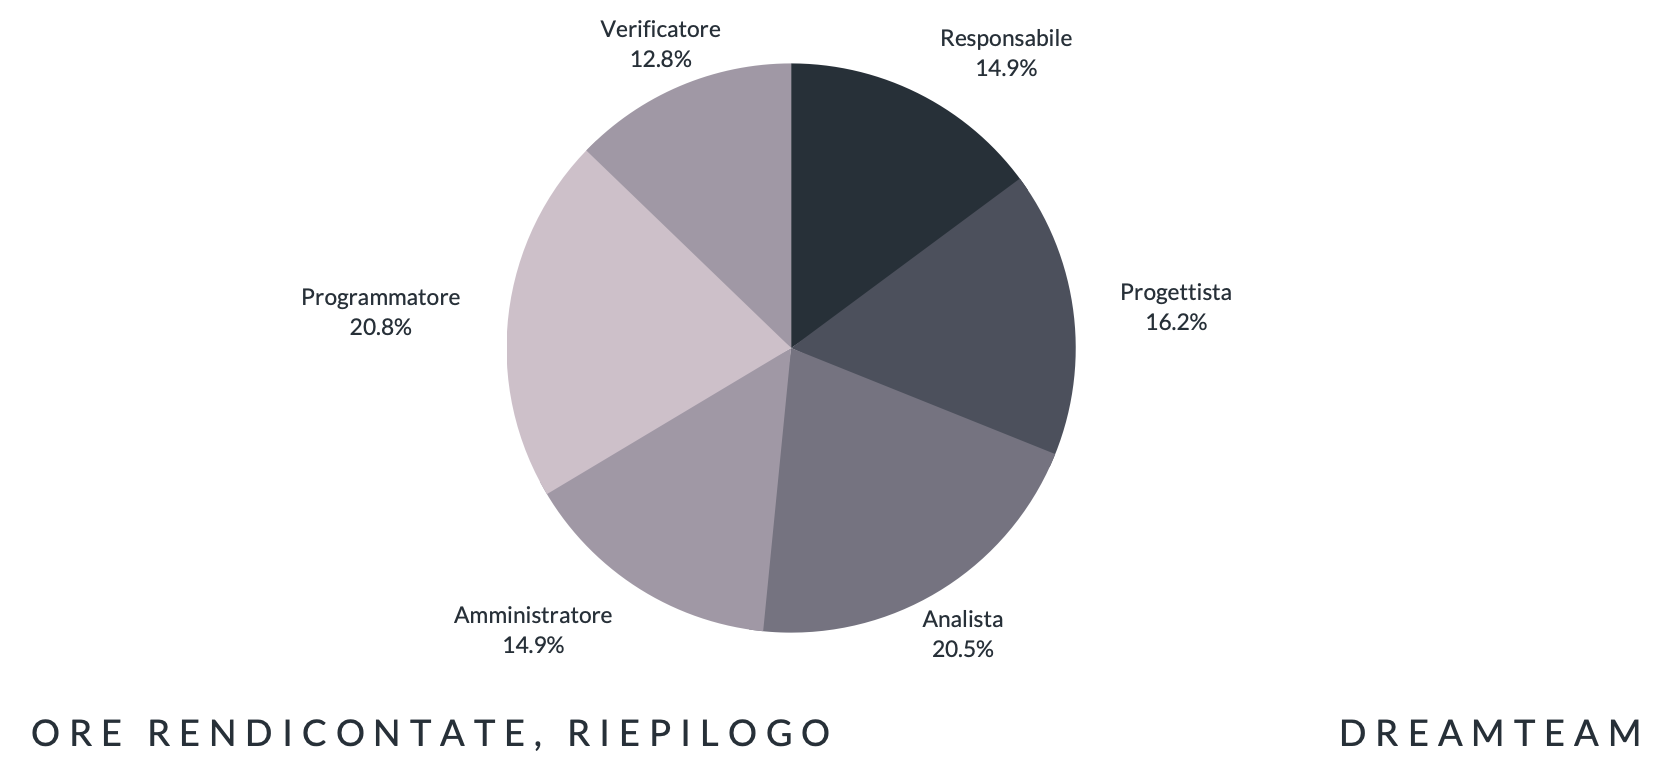
\includegraphics[scale=0.53]{Sezioni/SezioniPreventivo/grafici/Riepilogo_ore_totali_costi.png}
% \caption{Grafico a torta della ripartizione per ruolo delle ore totali}
% \end{figure}

\pagebreak


\subsection{Consuntivo totale v2}
\subsubsection{Prospetto orario}

La tabella seguente riporta il totale delle ore di lavoro effettivamente svolte dai singoli membri del gruppo durante il progetto, incluse le fasi di \textit{Analisi} e \textit{Produzione del Poof of Concept}.

\begin{table}[H]
	\begin{center}
	\rowcolors{2}{gray!25}{white}
	\renewcommand{\arraystretch}{1.25}
	\begin{tabular}{ m{0.20\textwidth}<{\centering}  m{0.06\textwidth}<{\centering} m{0.06\textwidth}<{\centering} m{0.06\textwidth}<{\centering}  m{0.06\textwidth}<{\centering}  m{0.06\textwidth}<{\centering}  m{0.06\textwidth}<{\centering}  m{0.20\textwidth}<{\centering}   }
		\rowcolor{darkblue}
		\textcolor{white}{\textbf{Componente}} &\textcolor{white}{\textbf{Re}}&\textcolor{white}{\textbf{Pt}}&\textcolor{white}{\textbf{An}}&\textcolor{white}{\textbf{Am}}&\textcolor{white}{\textbf{Pr}}&\textcolor{white}{\textbf{Ve}}&\textcolor{white}{\textbf{Ore complessive}}\\ 
		Edoardo Pavan & 10 & 14 & 10 & 11 & 15 & 20 & 80 \\	
		
		Francesco Protopapa & 10 & 10 & 20 & 5 & 35 & 20 & 100 \\
	
		Greta Cavedon & 15 & 10 & 20 & 4 & 26 & 25 & 100 \\
		
		Luciano Wu & 5 & 20 & 20 & 5 & 38 & 12 & 100 \\
		
		Matteo Basso & 5 & 15 & 12 & 8 & 35 & 25 & 100 \\
		
		Michele Gatto & 8 & 16 & 5 & 12 & 35 & 24 & 100 \\
		
		Pietro Villatora & 5 & 15 & 10 & 12 & 38 & 20 & 100 \\
		
		\textbf{Ore totali ruolo} & 58 & 100 & 97 & 57 & 222 & 146 & 680 \\
	
	\end{tabular}
	\caption{Distribuzione delle ore rendicontate}
	\end{center}
	\end{table}

\subsubsection{Prospetto economico}
La seguente tabella riporta i costi derivati dalle ore impiegate per ogni ruolo durante il progetto, incluse le fasi di \textit{Analisi} e \textit{Produzione del Poof of Concept}.

\begin{table}[H]
\begin{center}
\rowcolors{2}{gray!25}{white}
\renewcommand{\arraystretch}{1.5}
\begin{tabular}{ m{0.3\textwidth}<{\centering}  m{0.2\textwidth}<{\centering} m{0.2\textwidth}<{\centering}}
	\rowcolor{darkblue}
	\textcolor{white}{\textbf{Ruolo}}&\textcolor{white}{\textbf{Totale ore}}&\textcolor{white}{\textbf{Costo totale (\euro)}}\\ 

	Responsabile & 59(+1) & 1770(+30,00) \\	
	
	Progettista & 101(+1) & 2525(+25,00) \\
	
	Analista & 92(-5) & 2300(-125,00) \\

	Amministratore & 57(+0) & 1140(+0,00) \\
	
	Programmatore & 222(+0) & 3330(+0,00) \\
	
	Verificatore & 148(+2) & 2220(+30,00) \\
	
	\textbf{Totale} & 679(-1) & 13310(-15,00) \\
	
\end{tabular}
\caption{Prospetto dei costi totali delle ore complessive}
\end{center}
\end{table}

La tabella può essere rappresentata anche in forma visiva dal seguente aerogramma:

\subsubsection{Conclusioni}
Il gruppo chiude le attività di progetto con un bilancio positivo: 13310,00\euro, a fronte di un preventivo di 13325,00\euro. \\

La redazione di una pianificazione realistica e funzionale è stata un'attività molto complicata, poichè i membri del gruppo non erano abituati ad organizzare le attività di un progetto così ampio in termini di tempo. Non sorprende, quindi, che il \textit{Responsabile} e gli \textit{Amministratori} abbiano più volte dovuto riprendere in mano la pianificazione, soprattutto a seguito della prima valutazione da parte del committente. Tuttavia, il gruppo è riuscito a portare a termine tutte le attività previste, talvolta in anticipo rispetto a quanto pianificato.

La ripartizione delle ore tra i vari ruoli in alcuni incrementi si è rivelata poco adatta alle effettive esigenze del team, ad esempio nel III, IV e V incremento della fase di \textit{Progettazione e Codifica}, erano state preventivate alcune ore per l'analista che non sono state neccessarie e che sarebbero state necessarie in altri ruoli. Fortunatamente il gruppo ha deciso di non cambiare la pianificazione e utilizzare quel risparmio, sia di ore che di costi, per l'ultima fase. Nonostante queste piccole discrepanze il gruppo è riuscito a portare a termine il progetto senza portare il bilancio in negativo.

\begin{figure}[H]
\centering
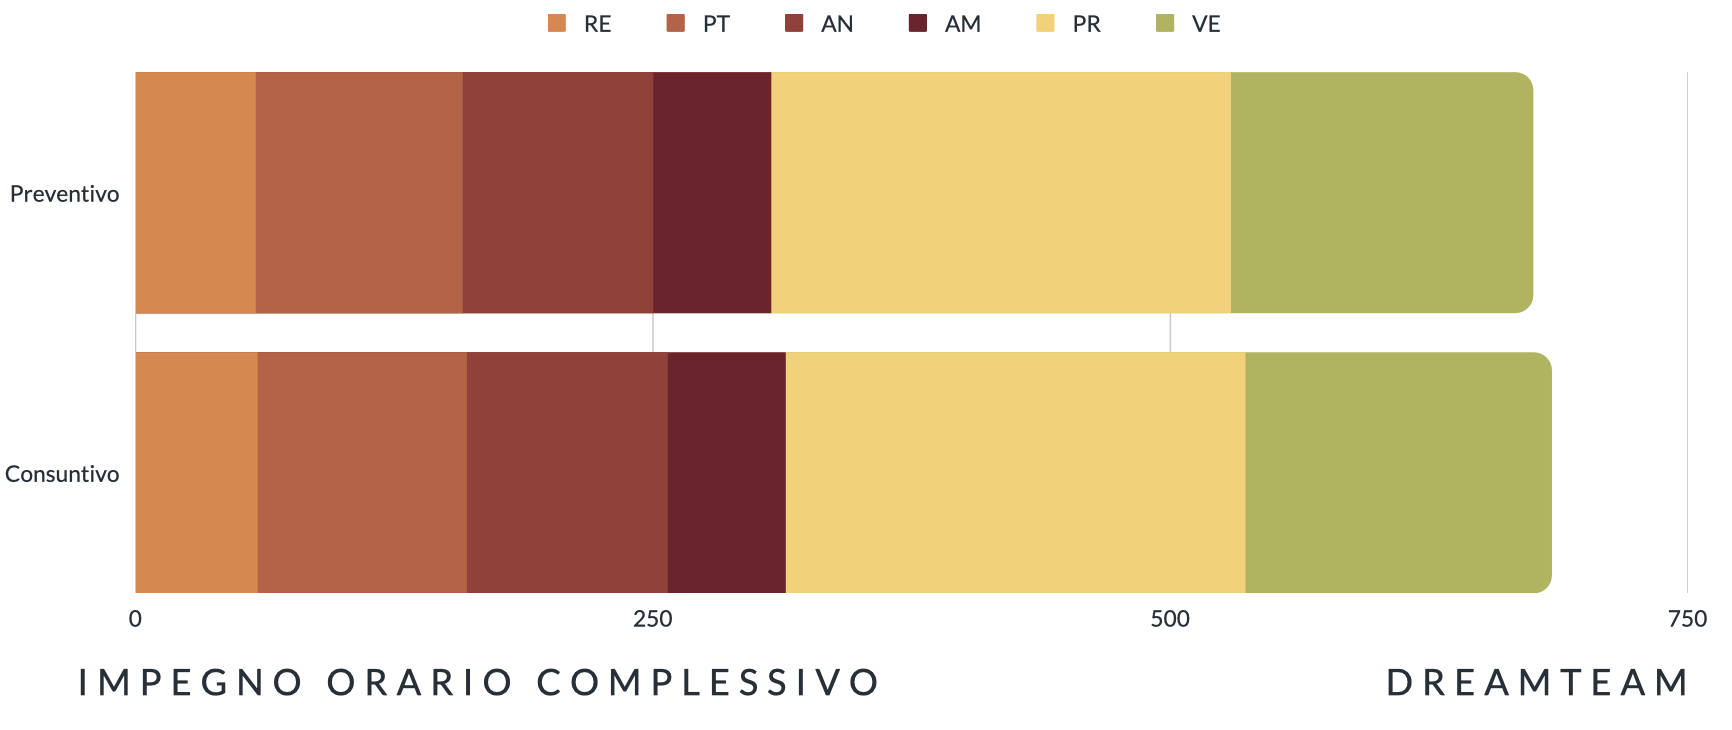
\includegraphics[scale=0.53]{Sezioni/SezioniPreventivo/grafici/Impegno_orario_complessivo.png}
\caption{Ripartizione delle ore totali ciascun ruolo, con confronto tra il preventivo e il consuntivo}
\end{figure}

In conclusione, il gruppo valuta positivamente il proprio lavoro, soprattutto trattandosi della prima esperienza per tutti i membri del gruppo \textit{DreamTeam}.



